\documentclass{article}
\usepackage[warn]{mathtext}
\usepackage[russian]{babel}
\usepackage[pdf]{graphviz}
\usepackage[utf8]{inputenc}
\usepackage[T2]{fontenc}
\usepackage{graphicx}
\graphicspath{ {images/} }

\title{ТМВ ДЗ №1}
\author{Каменев Руслан A-05-19}

\begin{document}
\maketitle
\section{Построить конечный автомат, распознающий язык}


    \quad 1. $L = \{w \in \{a, b, c\}^*  \; | \; |w|_c = 1\}$
    \begin{center}
        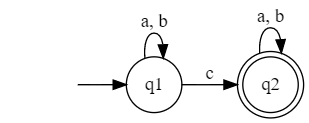
\includegraphics[width=0.4\textwidth]{task1/pic1.1}
    \end{center}
    \quad 2. $L = \{w \in \{a, b\}^* \; | \; |w|_a \leq 2, |w|_b \geq 2\}$
    \begin{center}
        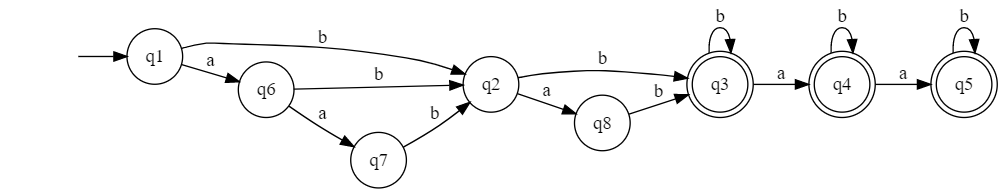
\includegraphics[width=0.8\textwidth]{task1/pic1.2}\\
    \end{center}
    \quad 3. $L = \{w \in \{a, b\}^* \; | \; |w|_a \neq |w|_b\}$
    \begin{center}
        \begin{alltt} 
        Для данного языка нельзя построить конечный автомат, т.к. нужно запомнимать количество символов ${a}$ и ${b}$ - чего конечные автоматы делать не умеют, но, кажется, конечные автоматы с магазинной памятью такое могут ... (но это неточно)
        \end{alltt}
    \end{center}
    \quad 4. $L = \{w \in \{a, b\}^* \; | \; ww = www\}$\\
    Этот язык будет состоят только из пустых цепочек ($|w| = 0$), т.к. \newline
    при $|w|>0\;ww \neq www$.
    \begin{center}
        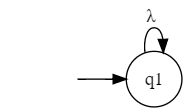
\includegraphics[width=0.3\textwidth]{task1/pic1.4}\\
    \end{center}
    
\section{Построить КА, используя прямое произведение}

    1. $L_1 = \{w \in \{a, b\}^* \; | \; |w|_a \geq 2 \wedge |w|_b \geq 2\}$\\
    Разобьем на 2 автомата:
    $$L_{11} = \{w \in \{a, b\}^* \; | \; |w|_a \geq 2\}, \quad L_{12} = \{w \in \{a, b\}^* \; | \; |w|_b \geq 2\}$$\\
    \begin{center}
        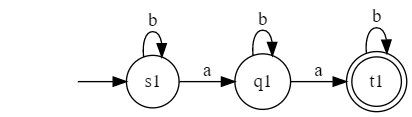
\includegraphics[width=0.45\textwidth]{task2/pic2.1.1}
        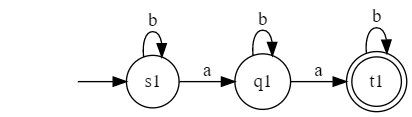
\includegraphics[width=0.45\textwidth]{task2/pic2.1.1}
    \end{center}
    $L_{11}=(\Sigma_1 = \{a, b\};\; Q_1 = \{s_1, q_1, t_1\};\; s_1;\; T_1 = \{q_1\}; \delta_1)$ \newline
    $L_{12}=(\Sigma_2 = \{a, b\};\; Q_2 = \{s_2, q_2, t_2\};\; s_2;\; T_2 = \{q_2\};
    \delta_1)$ \newline
    $A = L_{11} \land L_{12}$, по определению прямого произведения: \newline\newline
    $A = (\Sigma; Q; s; T; \delta)$, где: \newline
    $\Sigma = \Sigma_1 \land \Sigma_2 = (a, b)$ \newline
    $Q = Q_1 \times Q_2$ \newline
    $s = (s_1, s_2)$ \newline
    $T = T_1 \times T_2 = (q_1, q_2)$ \newline
    $\delta((s_1, s_2), a) = (\delta_1(s_1, a), \delta_2(s_2, a))$ \newline\newline
    Новые пвершины и переходы между ними:
    \begin{center}
        \begin{tabular}{|c|c|c|}
            \hline
            Сочетания точек & Переход по a & Переход по b \\
            \hline
            s_1s_2 & q_1s_2 & s_1q_2\\
            s_1q_2 & q_1q_2 & s_1t_2\\
            s_1t_2 & q_1t_2 & s_1t_2\\
            q_1s_2 & t_1s_2 & q_1q_2\\
            q_1q_2 & t_1q_2 & q_1t_2\\
            q_1t_2 & t_1t_2 & q_1t_2\\
            t_1s_2 & t_1s_2 & t_1q_2\\
            t_1q_2 & t_1q_2 & t_1t_2\\
            12 & 12 & 12\\
            \hline
        \end{tabular}\\
    \end{center}
    Получим:
    \begin{center}
        \includegraphics[width=0.9\textwidth]{task2/pic2.1.res}\\
    \end{center}
    
    2. $L_2 = \{w \in \{a, b\}^* \; | \; |w| \geq 3 \wedge |w|\;-\; нечёт\}$\\
    Разобьем на 2 автомата:
    $$L_{21} = \{w \in \{a, b\}^* \; | \; |w| \geq 3\}, \quad L_{22} = \{w \in \{a, b\}^* \; | \; |w|\quad odd\}$$
    \begin{center}
        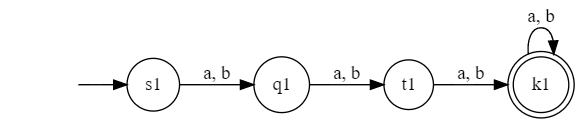
\includegraphics[width=0.5\textwidth]{task2/pic2.2.1}
        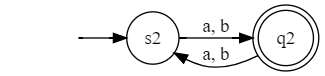
\includegraphics[width=0.4\textwidth]{task2/pic2.2.2}
    \end{center}
    $L_{21}=(\Sigma_1 = \{a, b\};\; Q_1 = \{s_1, q_1, t_1, k_1\};\; s_1;\; T_1 = \{k_1\}; \delta_1)$ \newline
    $L_{22}=(\Sigma_2 = \{a, b\};\; Q_2 = \{s_2, q_2\};\; s_2;\; T_2 = \{q_2\}; \delta_2)$ \newline
    $A = L_{21} \land L_{22}$, по определению прямого произведения: \newline\newline
    $A = (\Sigma; Q; s; T; \delta)$, где: \newline
    $\Sigma = \Sigma_1 \land \Sigma_2 = (a, b)$ \newline
    $Q = Q_1 \times Q_2$ \newline
    $s = (s_1, s_2)$ \newline
    $T = T_1 \times T_2 = (q_1, q_2)$ \newline
    $\delta((s_1, s_2), a) = (\delta_1(s_1, a), \delta_2(s_2, a))$ \newline\newline
    Новые пвершины и переходы между ними:
    \begin{center}
        \begin{tabular}{|c|c|c|}
            \hline
            Сочетания точек & Переход по a & Переход по b \\
            \hline
            s_1s_2 & q_1q_2 & q_1q_2\\
            s_1q_2 & q_1s_2 & q_1s_2\\
            q_1s_2 & t_1q_2 & t_1q_2\\
            q_1q_2 & t_1s_2 & t_1s_2\\
            t_1s_2 & k_1q_2 & k_1q_2\\
            t_1q_2 & k_1s_2 & k_1s_2\\
            k_2s_2 & k_1q_2 & k_1q_2\\
            k_1q_2 & k_1s_2 & k_1s_2\\
            \hline
        \end{tabular}\\
    \end{center}
    Получим:
    \begin{center}
        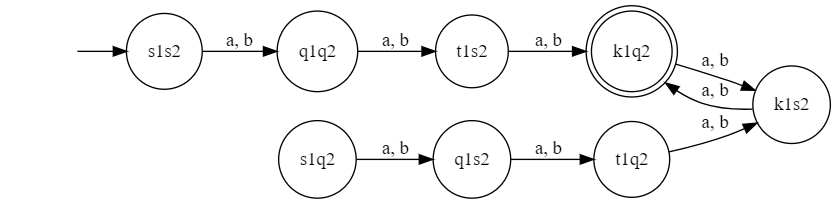
\includegraphics[width=0.9\textwidth]{task2/pic2.2res}\\
    \end{center}
    Так как в вершину $s_1q_2$ попасть нельзя, можно автомат немного упростить:
    \begin{center}
        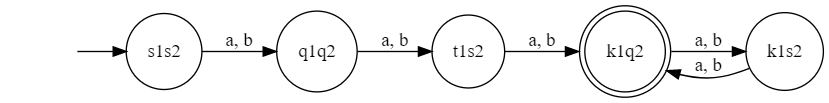
\includegraphics[width=0.9\textwidth]{task2/pic2.2res(simplier)}\\
    \end{center}
    
    3. $L_3 = \{w \in \{a, b\}^* \; | \; |w|_a - чёт \wedge |w|_b - кратно\;3\}$\\
    Разобьем на 2 автомата:
    $$L_{31} = \{w \in \{a, b\}^* \; | \; |w|_a - чёт\}, \quad L_{32} = \{w \in \{a, b\}^* \; | \; |w|_b- кратно\;3\}$$
    \begin{center}
        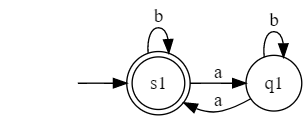
\includegraphics[width=0.4\textwidth]{task2/pic3.1}
        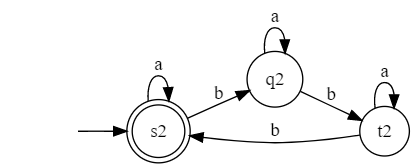
\includegraphics[width=0.5\textwidth]{task2/pic3.2}
    \end{center}
    $L_{31}=(\Sigma_1 = \{a, b\};\; Q_1 = \{s_1, q_1\};\; s_1;\; T_1 = \{s_1\}; \delta_1)$ \newline
    $L_{32}=(\Sigma_2 = \{a, b\};\; Q_2 = \{s_2, q_2, t_2\};\; s_2;\; T_2 = \{s_2\}; \delta_2)$ \newline
    $A = L_{31} \land L_{32}$, по определению прямого произведения: \newline\newline
    $A = (\Sigma; Q; s; T; \delta)$, где: \newline
    $\Sigma = \Sigma_1 \land \Sigma_2 = (a, b)$ \newline
    $Q = Q_1 \times Q_2$ \newline
    $s = (s_1, s_2)$ \newline
    $T = T_1 \times T_2 = (s_1, s_2)$ \newline
    $\delta((s_1, s_2), a) = (\delta_1(s_1, a), \delta_2(s_2, a))$ \newline\newline
    Новые пвершины и переходы между ними:
    \begin{center}
        \begin{tabular}{|c|c|c|}
            \hline
             Сочетания точек & Переход по a & Переход по b  \\
            \hline
            s_1s_2 & q_1s_2 & s_1q_2\\
            s_1q_2 & q_1q_2 & s_1t_2\\
            s_1t_2 & q_1t_2 & s_1s_2\\
            q_1s_2 & s_1s_2 & q_1q_2\\
            q_1q_2 & s_1t_2 & q_1t_2\\
            q_1t_2 & s_1t_2 & q_1s_2\\
            \hline
        \end{tabular}\\
    \end{center}
    Получим:
    \begin{center}
        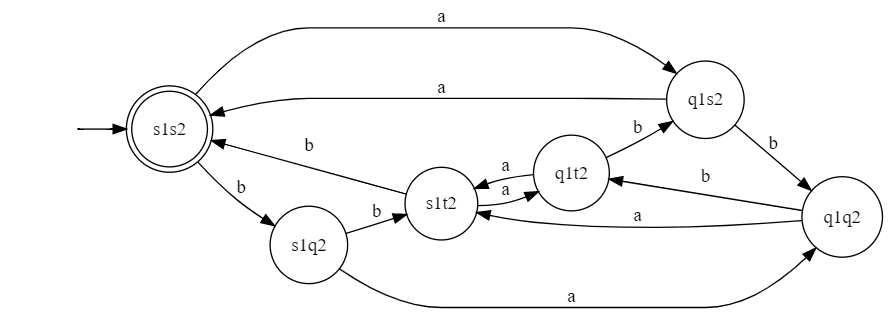
\includegraphics[width=0.9\textwidth]{task2/pic3.3}
    \end{center}
    
    
    4. $L_4 = \overline{L_3}$\\
    Чтобы построить отрицание, нужно инвертировать терминальные и нетерминальные вершины:
    \begin{center}
        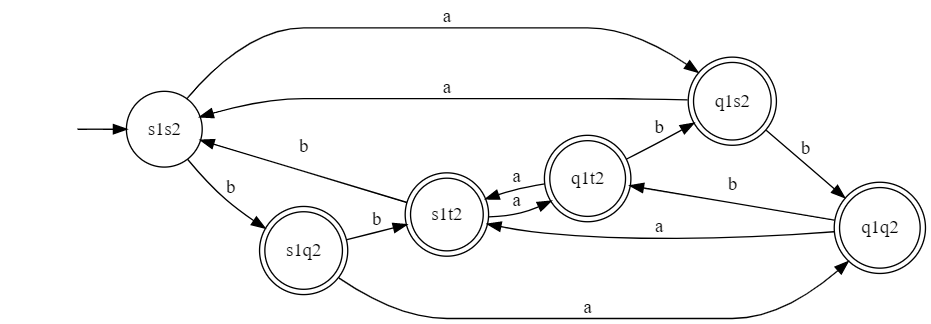
\includegraphics[width=0.9\textwidth]{task2/pic3.4}
    \end{center}
    
    5. $L_5 = L_2 \setminus L_3 = L_2 \wedge L_4 $\\
    Найдём пересечение двух языков:
    \begin{center}
        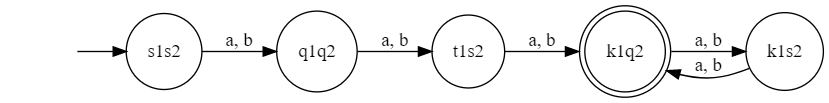
\includegraphics[width=0.9\textwidth]{task2/pic2.2res(simplier)}
        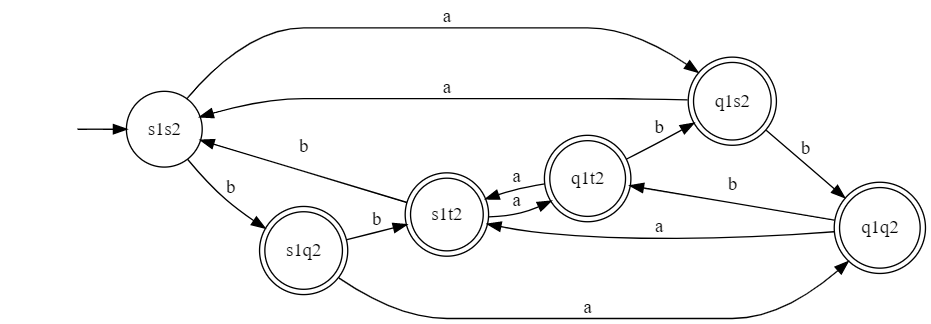
\includegraphics[width=0.9\textwidth]{task2/pic3.4}
    \end{center}
    Выполнив переобозначение вершин, получим: \newline
    \begin{center}
        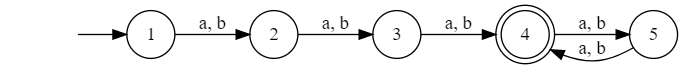
\includegraphics[width=0.9\textwidth]{task2/pic5.1}
        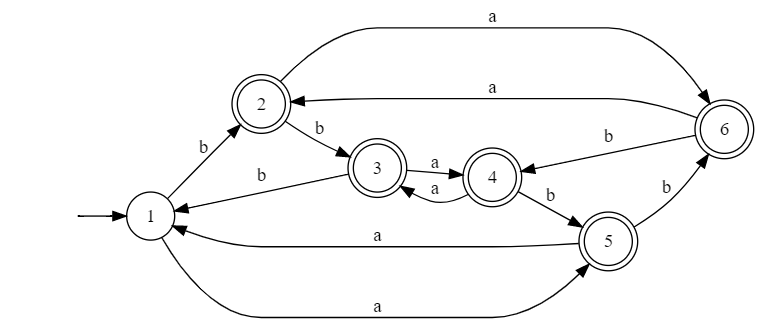
\includegraphics[width=0.9\textwidth]{task2/pic5.2}
    \end{center}
    $L_5 = L_2 \wedge L_4$. Имеем $\Sigma = \{a, b\}, s = 11, T = 42$.
    Новые пвершины и переходы между ними:
    \begin{center}
        \begin{tabular}{|c|c|c|}
            \hline
            Сочетания точек & Переход по a & Переход по b \\
            \hline
            11 & 25 & 22\\
            12 & 26 & 23\\
            13 & 24 & 21\\
            14 & 23 & 25\\
            15 & 21 & 26\\
            16 & 22 & 24\\
            21 & 35 & 32\\
            22 & 36 & 33\\
            23 & 34 & 31\\
            24 & 33 & 35\\
            25 & 31 & 36\\
            26 & 32 & 34\\
            31 & 45 & 42\\
            32 & 46 & 43\\
            33 & 44 & 41\\
            34 & 43 & 45\\
            35 & 41 & 46\\
            36 & 42 & 44\\
            41 & 55 & 52\\
            42 & 56 & 53\\
            43 & 54 & 51\\
            44 & 53 & 55\\
            45 & 51 & 56\\
            46 & 52 & 54\\
            51 & 45 & 62\\
            52 & 46 & 43\\
            53 & 44 & 41\\
            54 & 43 & 45\\
            55 & 41 & 46\\
            56 & 42 & 44\\
            \hline
        \end{tabular}\\
    \end{center}
    Получим:
    \begin{center}
        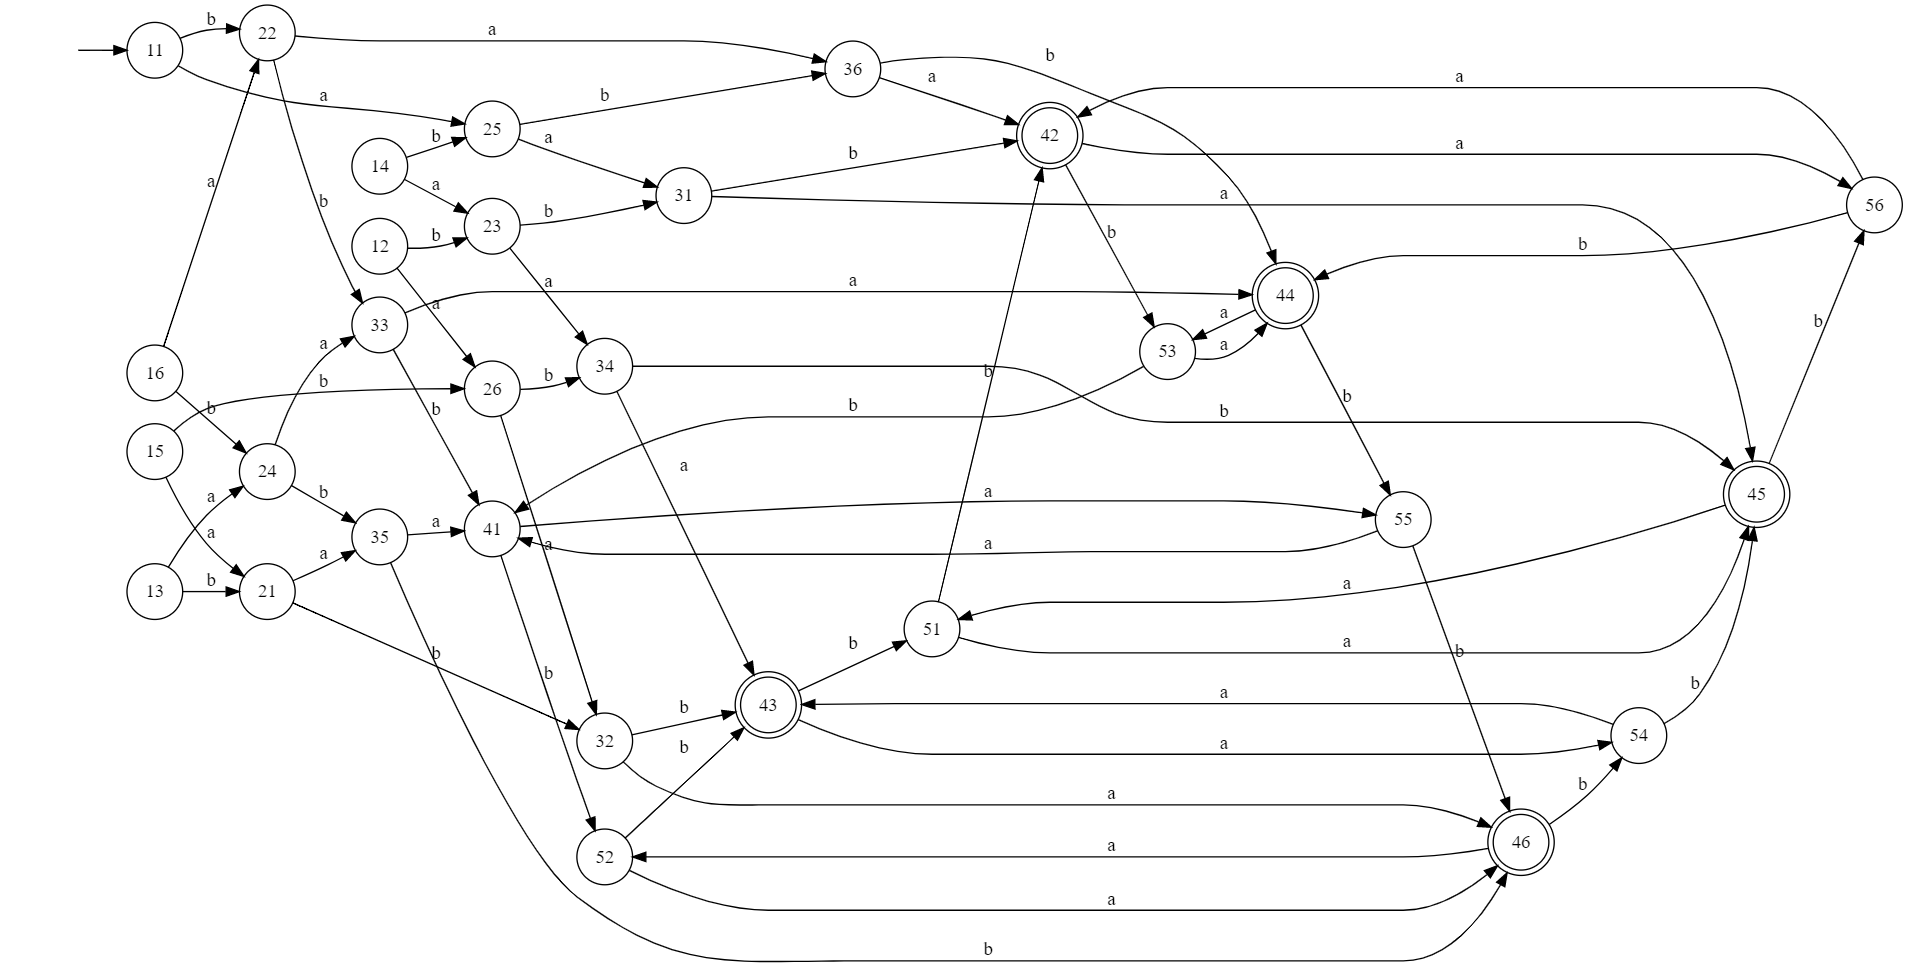
\includegraphics[width=1\textwidth]{task2/pic5.3}\\
    \end{center}
    
\end{document}
© 2022 GitHub, Inc.
Terms
Privacy
Security
Status
Docs
Contact GitHub
Pricing
API
Training
Blog
About

